\PassOptionsToPackage{unicode=true}{hyperref} % options for packages loaded elsewhere
\PassOptionsToPackage{hyphens}{url}
%
\documentclass[]{article}
\usepackage{lmodern}
\usepackage{amssymb,amsmath}
\usepackage{ifxetex,ifluatex}
\usepackage{fixltx2e} % provides \textsubscript
\ifnum 0\ifxetex 1\fi\ifluatex 1\fi=0 % if pdftex
  \usepackage[T1]{fontenc}
  \usepackage[utf8]{inputenc}
  \usepackage{textcomp} % provides euro and other symbols
\else % if luatex or xelatex
  \usepackage{unicode-math}
  \defaultfontfeatures{Ligatures=TeX,Scale=MatchLowercase}
\fi
% use upquote if available, for straight quotes in verbatim environments
\IfFileExists{upquote.sty}{\usepackage{upquote}}{}
% use microtype if available
\IfFileExists{microtype.sty}{%
\usepackage[]{microtype}
\UseMicrotypeSet[protrusion]{basicmath} % disable protrusion for tt fonts
}{}
\IfFileExists{parskip.sty}{%
\usepackage{parskip}
}{% else
\setlength{\parindent}{0pt}
\setlength{\parskip}{6pt plus 2pt minus 1pt}
}
\usepackage{hyperref}
\hypersetup{
            pdftitle={Figures for SAPFLUXNET data paper},
            pdfauthor={R. Poyatos},
            pdfborder={0 0 0},
            breaklinks=true}
\urlstyle{same}  % don't use monospace font for urls
\usepackage[margin=1in]{geometry}
\usepackage{graphicx,grffile}
\makeatletter
\def\maxwidth{\ifdim\Gin@nat@width>\linewidth\linewidth\else\Gin@nat@width\fi}
\def\maxheight{\ifdim\Gin@nat@height>\textheight\textheight\else\Gin@nat@height\fi}
\makeatother
% Scale images if necessary, so that they will not overflow the page
% margins by default, and it is still possible to overwrite the defaults
% using explicit options in \includegraphics[width, height, ...]{}
\setkeys{Gin}{width=\maxwidth,height=\maxheight,keepaspectratio}
\setlength{\emergencystretch}{3em}  % prevent overfull lines
\providecommand{\tightlist}{%
  \setlength{\itemsep}{0pt}\setlength{\parskip}{0pt}}
\setcounter{secnumdepth}{0}
% Redefines (sub)paragraphs to behave more like sections
\ifx\paragraph\undefined\else
\let\oldparagraph\paragraph
\renewcommand{\paragraph}[1]{\oldparagraph{#1}\mbox{}}
\fi
\ifx\subparagraph\undefined\else
\let\oldsubparagraph\subparagraph
\renewcommand{\subparagraph}[1]{\oldsubparagraph{#1}\mbox{}}
\fi

% set default figure placement to htbp
\makeatletter
\def\fps@figure{htbp}
\makeatother


\title{Figures for SAPFLUXNET data paper}
\author{R. Poyatos}
\date{27/12/2019}

\begin{document}
\maketitle

\hypertarget{figures}{%
\subsection{Figures}\label{figures}}

\hypertarget{main-text}{%
\subsubsection{Main text}\label{main-text}}

This version of the figures use a low quality version of the base maps
because it's faster to run this way. Inaccuracies in the map result from
rasterisation.

\pagebreak

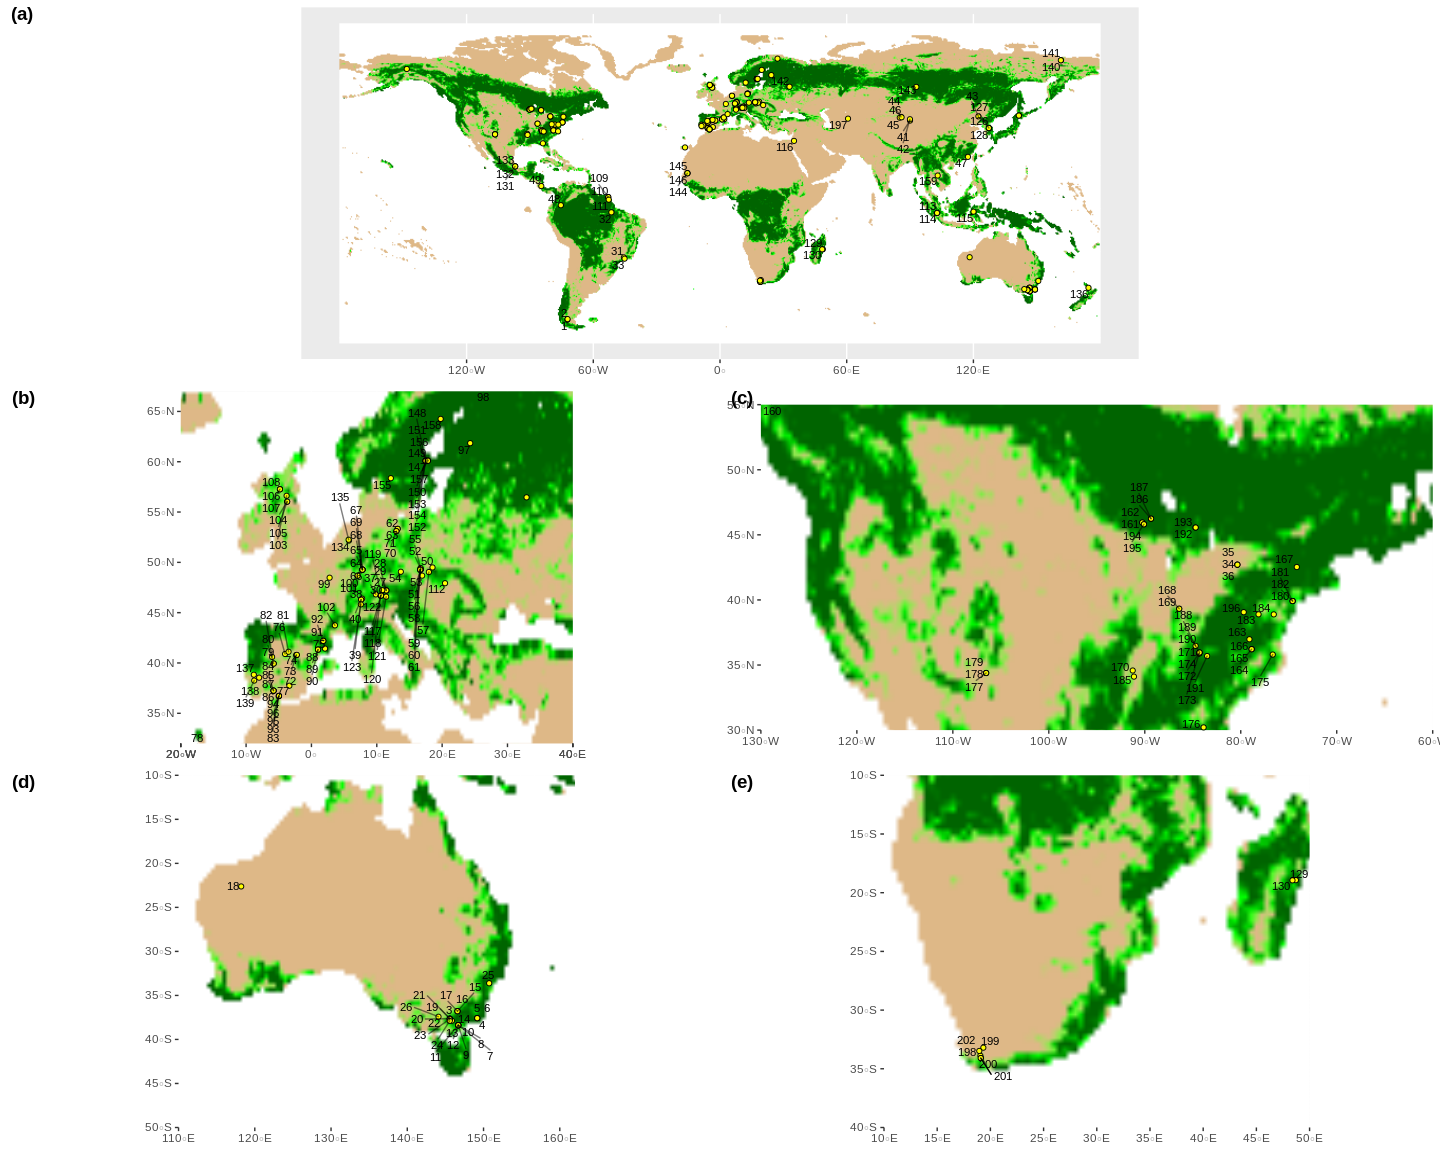
\includegraphics{figures_draft_files/figure-latex/sitesmap-1.pdf}

Figure 1. Geographical distribution of SAPFLUXNET datasets showing
dataset \#.

\pagebreak

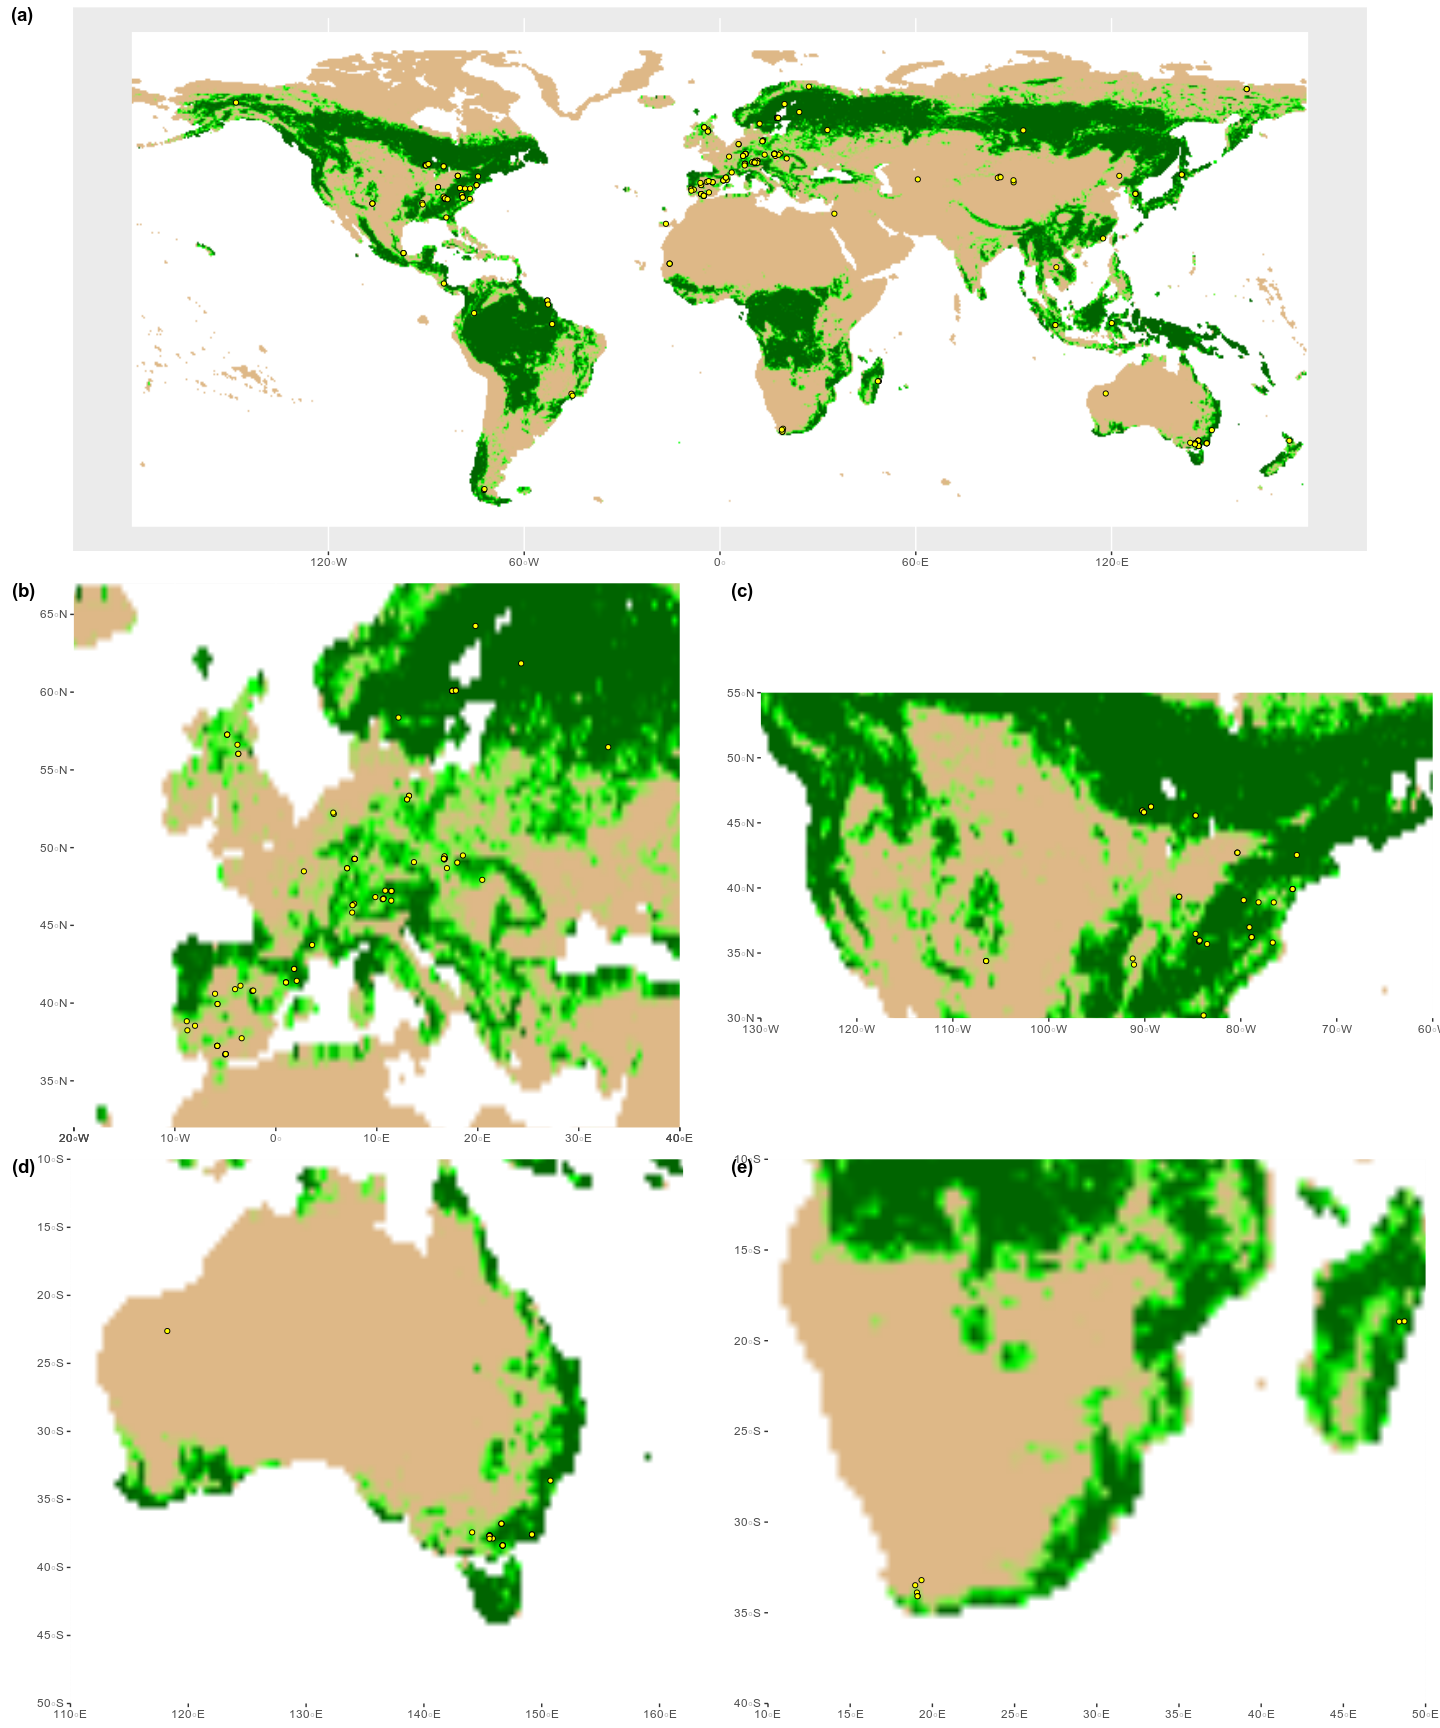
\includegraphics{figures_draft_files/figure-latex/sitesmap_nocodes-1.pdf}

Figure 1. Geographical distribution of SAPFLUXNET datasets.

\pagebreak

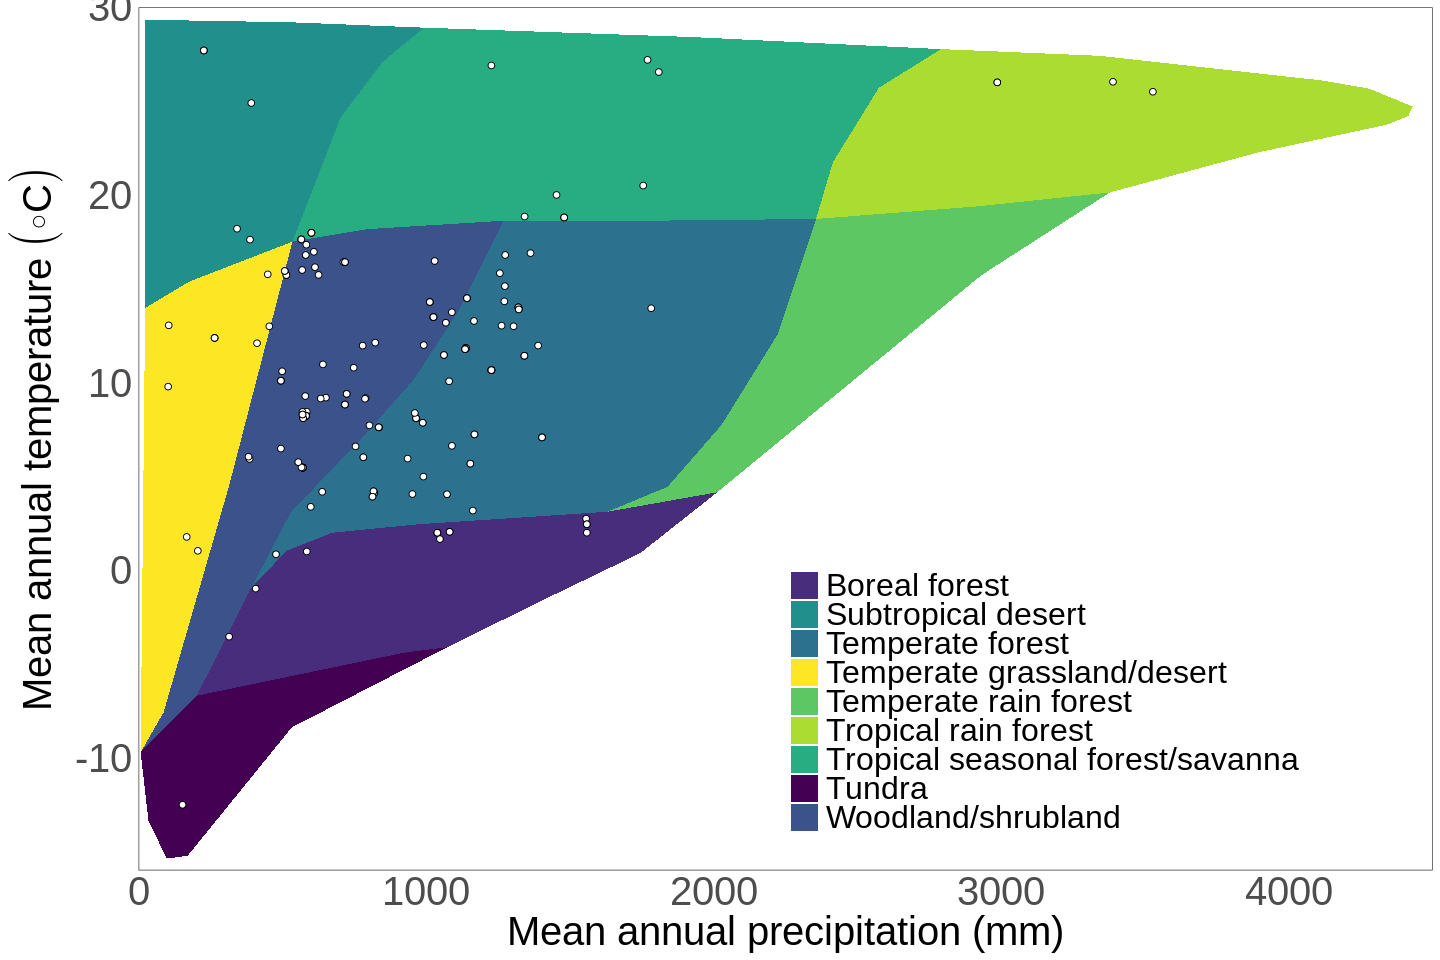
\includegraphics{figures_draft_files/figure-latex/biomemap-1.pdf} Figure
2. Bioclimatic distribution of SAPFLUXNET datasets in the Whittaker
biome space.

\pagebreak

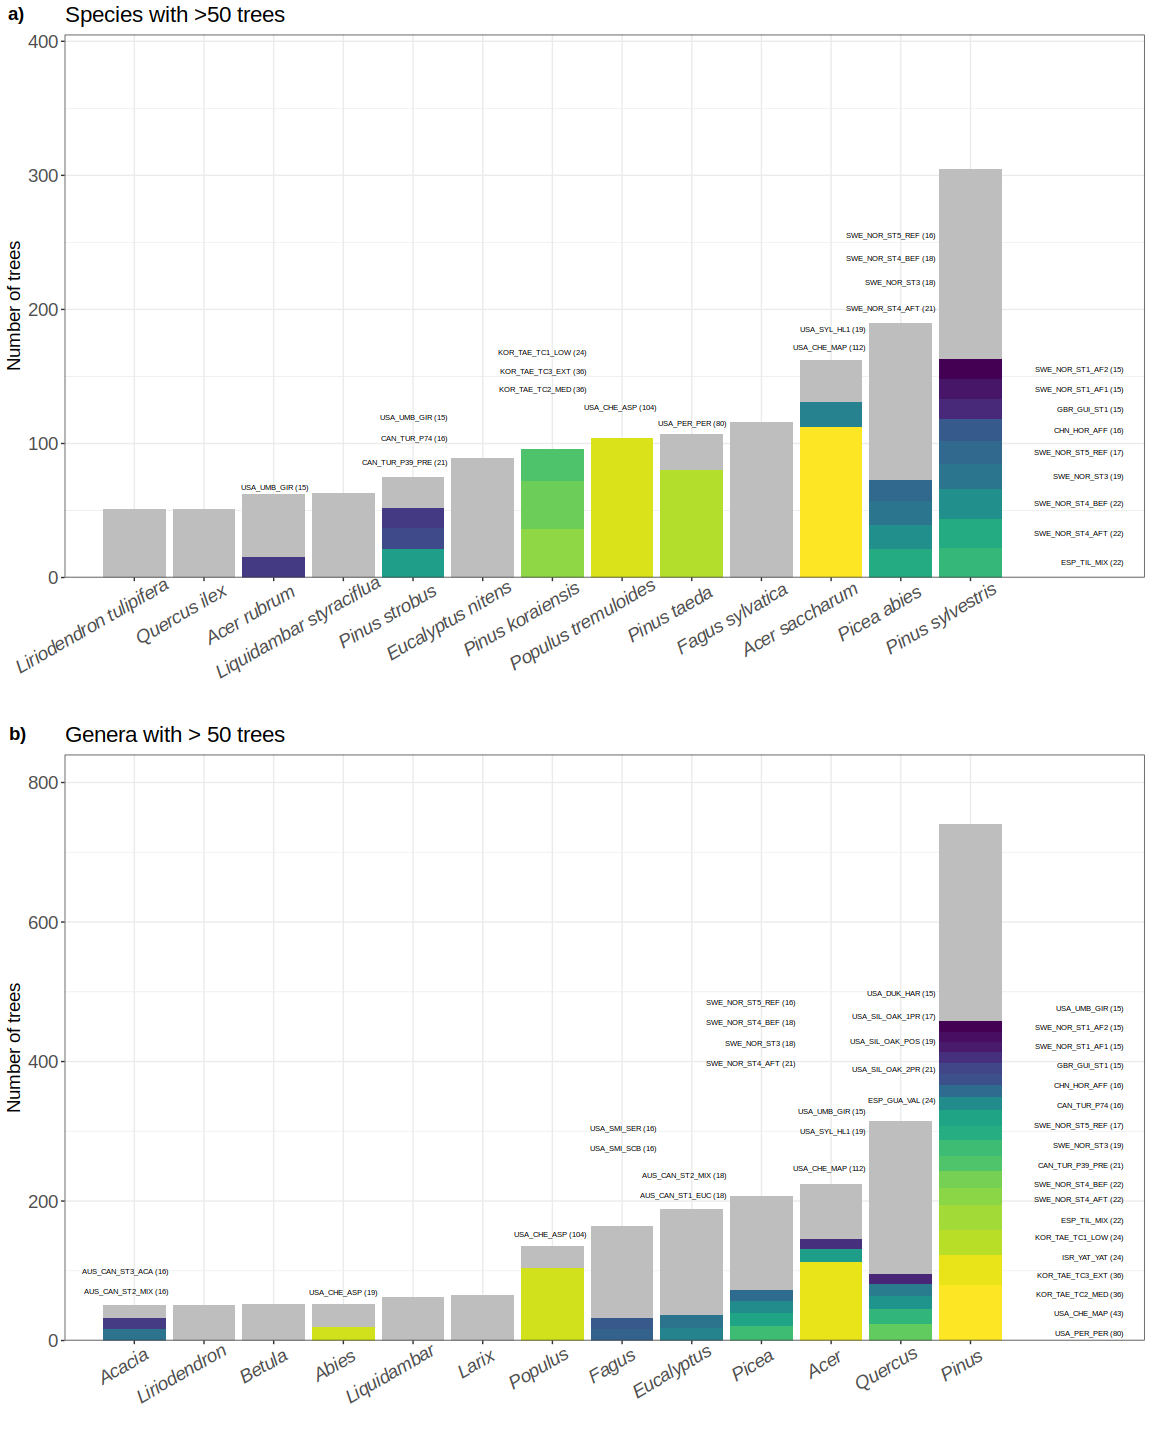
\includegraphics{figures_draft_files/figure-latex/genera_species-1.pdf}
Figure 3. Taxonomic distribution of genera and species in SAPFLUXNET,
showing (a) genera with \textgreater{} 50 trees and (b) species with
\textgreater{} 30 trees in the database.

\pagebreak

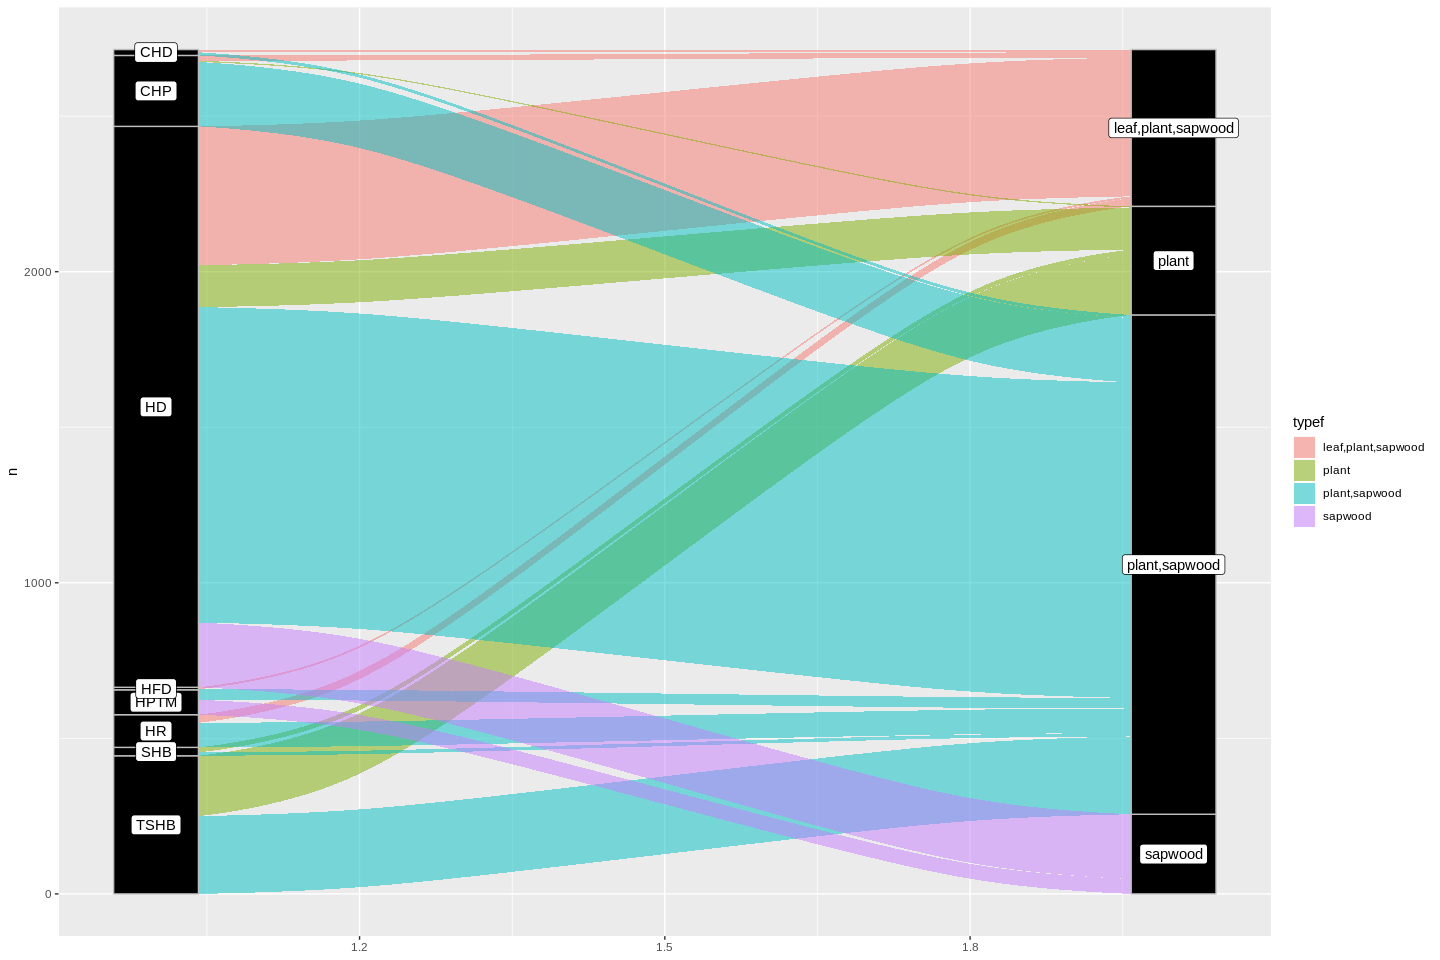
\includegraphics{figures_draft_files/figure-latex/method_type-1.pdf}

\end{document}
